%\section{Cold Rydberg gases as experimental platform}
\section{Using cold Rydberg gases to probe thermalization}\label{sec:Rydberg-experiment}
%highly excited atomic states, like small dipoles  (bar magnets) with quantum properties
%
%highly tunable, long-coherence times
%
%Rydberg blockade, tunable disorder

% quantum simulation \cite{georgescuQuantumSimulation2014}

Rydberg atoms, i.e., atoms in highly excited, hydrogen-like states, are a versatile platform for quantum simulation experiments due to their long coherence times and high degree of tunability~\cite{whitlockSimulatingQuantumSpin2017,sibalicRydbergPhysics2018,browaeysManybodyPhysicsIndividually2020a,schollQuantumSimulation2D2021}. The particular setup considered in this thesis does not employ tweezers, i.e. small traps for single atoms that can be manipulated individually, but instead traps a large amount of $^{87}$Rb atoms as a thermal cloud. The subsequent Rydberg excitation thus produces a different spatial configuration in each run of the experiment. This has the down-side that local control is very limited. However, the great advantage of this setup is the larger number of Rydberg atoms, which can well be in the thousands, in comparison to experiments using tweezers, which top out at a few hundreds of Rydberg atoms~\cite{browaeysManybodyPhysicsIndividually2020a}.

Using two different Rydberg states to encode the spin-$\frac{1}{2}$ degrees of freedom, this experiment naturally realizes a Heisenberg XXZ model~\cite{pineiroorioliRelaxationIsolatedDipolarInteracting2018,signolesGlassyDynamicsDisordered2021}
\begin{equation}\label{eq:heisenberg-hamiltonian}
	H = \sum_{i<j} J_{ij}\left(S_x^{(i)}S_x^{(j)} + S_y^{(i)}S_y^{(j)} + \Delta S_z^{(i)}S_z^{(j)}\right).
\end{equation}
Here the interactions $J_{ij}\propto |r_i-r_j|^{-\alpha}$ decay as power-law of the spatial separation with $\alpha=3$ (dipole-dipole) or $\alpha=6$ (van der Waals) depending on the chosen states (cf. Fig.~\ref{fig:experimental-hamiltonians}).

\begin{figure}[htb]
	\centering
	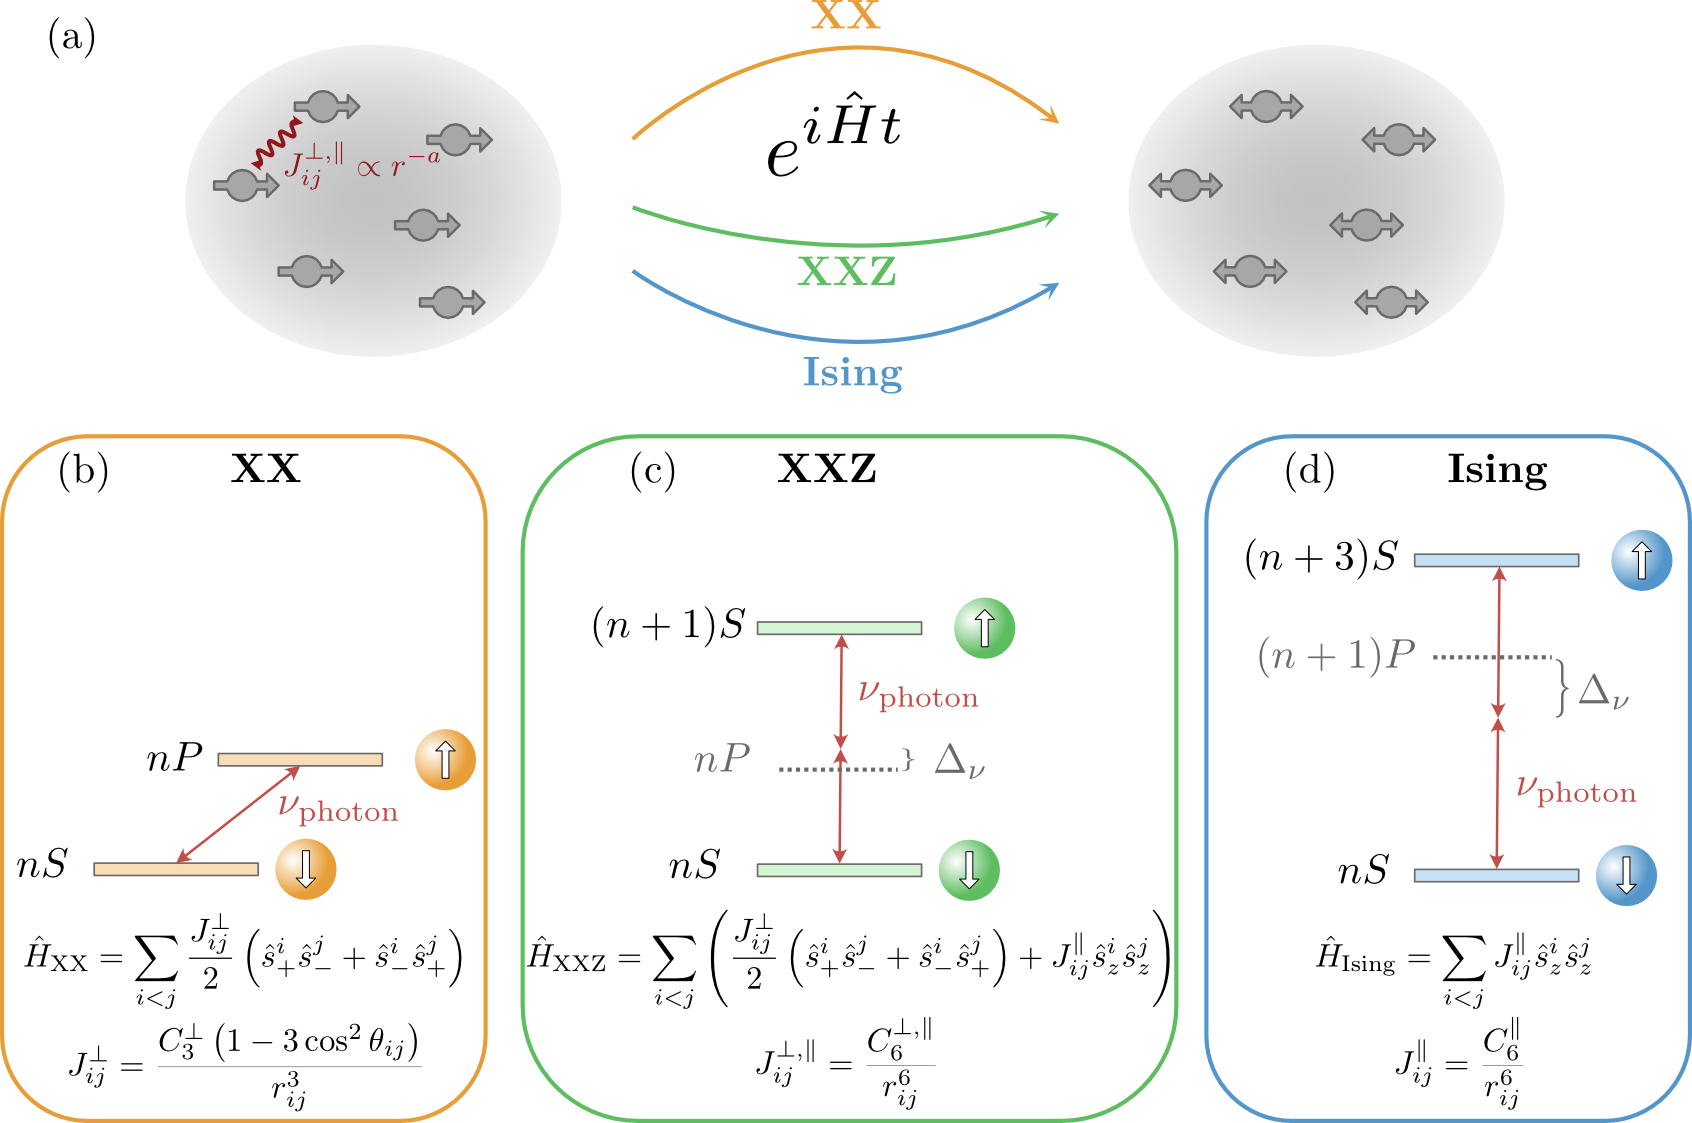
\includegraphics[width=\textwidth]{gfx/part1/png/experiment_hamiltonians.png}
	\caption{Schematic overview of the experimental features. (a) Spins are randomly distributed in space and feature power-law interactions and can evolve under different Heisenberg Hamiltonians. Depending on the choice of states, the experiment can realize XX (b), XXZ (c) and Ising (d) models.
		Adapted from~\cite{franzObservationAnisotropyindependentMagnetization2024}.}
	\label{fig:experimental-hamiltonians}
\end{figure}

While the Rydberg atoms are positioned randomly in each shot, there is a way to control the strength of the randomness. This is enabled by the Rydberg blockade, which shifts the Rydberg excitation of a groundstate atom off resonances if another Rydberg atom is close by\cite{lukinDipoleBlockadeQuantum2001}. Thus Rydberg atoms effectively enforce a certain minimal distance $r_b$ among them. Thus tuning the mean interspin distance $a_0$, which is related to the sample's density, we can manipulate the width of the coupling distribution (cf. Fig.~\ref{fig:disorder-distribution}). Concretely, for high density the spins need to pack tight and there is simply no room for large variations of the nearest neighbor distance. Conversely, at very low densities there is almost no correlation in the spin's locations.

\begin{figure}[htb]
	% TODO
	\centering
	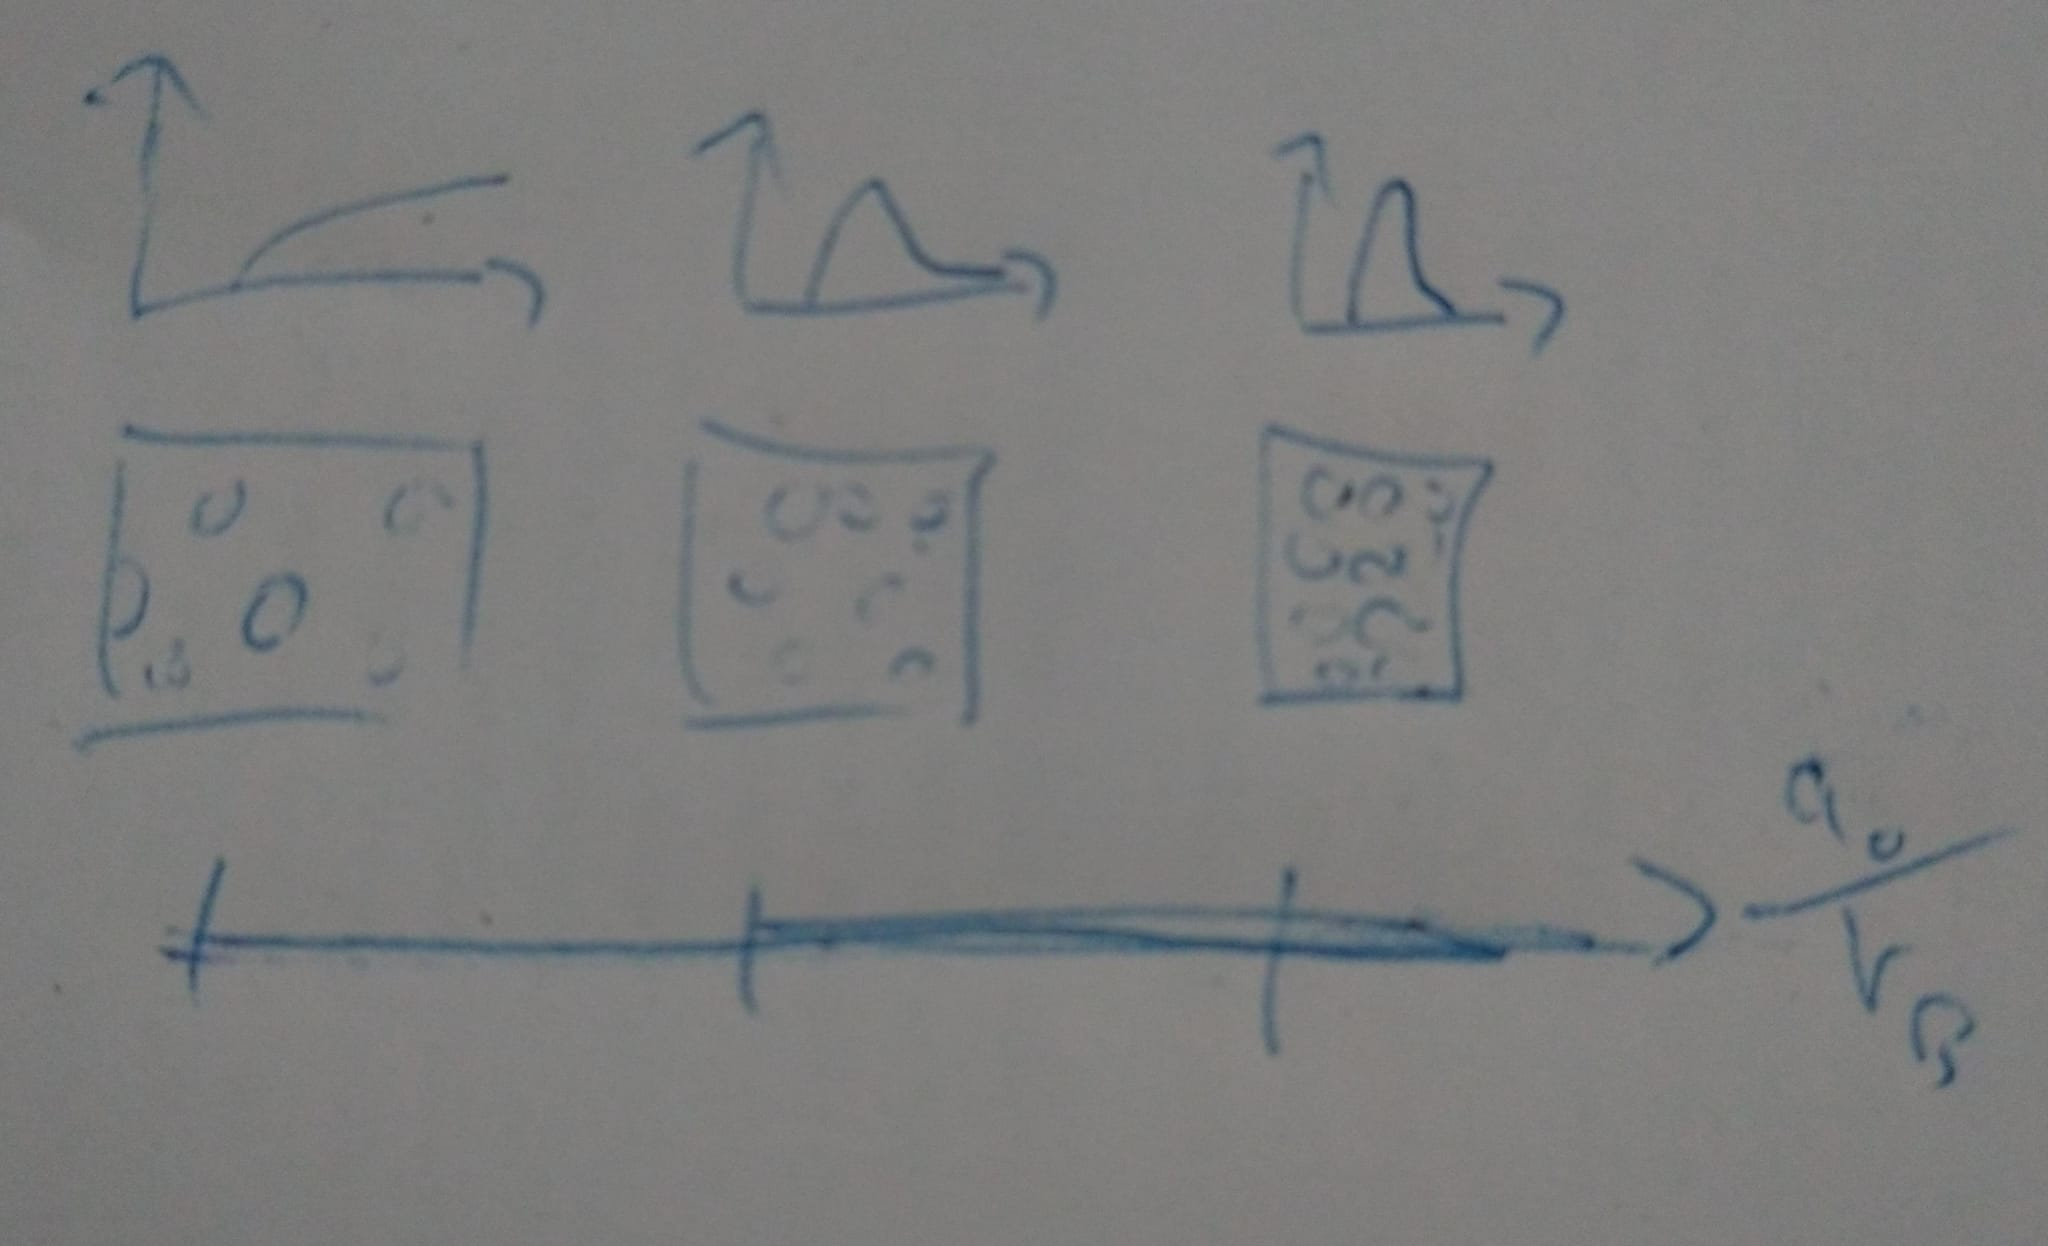
\includegraphics[width=\textwidth]{gfx/part1/experimental-disorder-strength.jpeg}
	\caption{Increasing density reduces the randomness in the distances by forcing atoms closer together. This modifies the coupling distributions.}
	\label{fig:disorder-distribution}
\end{figure}

In summary, this Rydberg quantum simulator allows for the exploration of different Heisenberg-type models with different interaction power-law exponents and tunable disorder strength all within the same experiment. 
